\documentclass[12pt, letterpaper, twoside]{report}
\usepackage[utf8]{inputenc}
\usepackage{graphicx}
\usepackage{mathtools}
\usepackage[margin=1in]{geometry}
\usepackage{amsmath}
\usepackage{setspace}
\usepackage{wrapfig}
\doublespacing
\newcommand*\mycommand[1]{\texttt{\emph{#1}}}
\bibliographystyle{ieeetr}
\title{Magnetic Effects in Metal Nanoparticle Arrays}
\author{Nicholas P. Montoni}
\date{\center{Wednesday, August 16, 2017\\Chemistry Building 339, 9:30 AM}}

\begin{document}

\begin{titlepage}
\maketitle
\end{titlepage}

%%%%%%%%%%%%%%%%%%%%%%%%%%%%%%%%%%%%%%%%%%%%%%%%%%%%%%%%%%%%%%%%%%%%%
%% Start the main part of the manuscript here.
%%%%%%%%%%%%%%%%%%%%%%%%%%%%%%%%%%%%%%%%%%%%%%%%%%%%%%%%%%%%%%%%%%%%%
\section*{Introduction}
Interest in the collective magnetic response of arrays of metal nanoparticles, called magnetic oligomers, has exploded in recent years. This is due to the possibility of applying magnetic plasmon resonances to problems such as biological sensing and imaging, electromagnetic cloaking, and information processing\cite{Zia2010trans,Noginova2008trans,Wang:13,Fan2015,Wei2015,Shvets2012,Altug2012bio,Nord2011fano,Zhang2006,NordHal2011,NordHal2012}. Plasmonic systems exhibiting magnetic properties have been thoroughly characterized on both the single-oligomer scale and the infinite scale, but open questions remain about the properties and usefulness of magnetic oligomers in the size regime between these two limits\cite{Dionne2016,Weick2013,Engheta2017}. Emphasizing this point is a wealth of research focusing on large, multi-oligomer arrays of nanoparticles. In particular, one such work highlights the complexity of these systems and sets the stage for the tunability and usefulness of magnetic plasmon resonances.

The recent work in question focused on describing one-, two-, and six-oligomer systems using both a quasistatic tight-binding model and full-wave simulations. The quasistatic approximation assumes that an object is so small that light and information travel across it infinitely quickly, or at least faster than the lifetime of any relevant physical phenomenon, such as a plasmon resonance. This is important to note because the formulation of the model is therefore fundamentally different from the simulations; the simulations include retardation effects. So it comes as no surprise that the model and the simulations predicted different properties for the two- and six-oligomer systems. The discrepancy occurred in the spectral ordering of the closed-loop magnetic modes: the tight-binding model predicted that the nodeless magnetic mode was higher in energy while simulations predicted that it was lower in energy. This discrepancy is a clear indication that the quasistatic approximation breaks down for magnetic systems and that retardation effects are in fact necessary to proeprly describe them.



When two or more metal nanoparticles (MNPs) are allowed to interact, the collective excitations of their conduction electrons, called electric plasmons, can hybridize to produce new excitations\cite{Lucas1976,ARAVIND1981,Xu1995,Mischenko1995}. Arranging three or more MNPs on the vertices of a polygon generates a collective mode that resembles a fictitious current loop and produces a magetic moment in the center of the polygon\cite{Alu2006,Alu2008,Liu2011,Nord2006,Cherqui2014}. Of recent interest has been the ability of magnetic plasmons, much like electric plasmons, to hybridize\cite{Cherqui2016}. Much work has been done to describe magnetic plasmons both in the single oligomer limit\cite{}, where the aggregates are well-described by the quasistatic approximation, and in the infinite limit, where extended systems are well-defined by condensed matter approaches\cite{}. In between these limits, however, there are still open questions about how to think about magnetic plasmons and what models work best\cite{}. 

Work that has attempted to describe finite arrays of magnetic oligomers within the quasistatic limit has had its limitations\cite{Cherqui2014}. Making the approximation that magnetic oligomers are small compared to the speed of light results in good qualitative analysis but lacks in quantitative accuracy when compared with full-wave electrodynamics simulations. Specifically, the quasistatic model predicted the wrong spectral order of the closed loop magnetic modes of two- and six-ring oligomers. This was corrected in a coarse-grained model, but the question remains of what the quasistatic model needed to predict the correct energy-ordering. Because the simulations use the fully-retarded formulation of Maxwell's equations, this work will use retardation effects to augment the simple model used previously in order to achieve quantitative accuracy and to explain why the quasistatic approximation is not accurate for magnetic oligomers. Retardation effects have been considered in studies of both large MNPs and infinite MNP arrays\cite{Abajo2008,Gu2010,vonPlessen2007,Rechbacher2003,Kottman2001,Schatz2003,Royer2005,Chumanov2010}, but have not yet been used to describe the optical properties of magnetic oligomers.

Beyond investigating previous work, the intuition gained from the simple model will be applied to suggest and explore applications and observables of magnetic plasmon oligomers. Specifically, because these aggregates can couple to and enhance the magnetic field of light, and because of their unique radiative properties, magnetic oligomers have applications such as solar cell enhancement\cite{Graydon2011,Alu2014solar,Le2015solar}, biosensing and detection\cite{}. This paper documents those unique properties and leverages them as a measure of the importance of retardation effects. As a final exercise, two explanations for these properties are proposed in order to gain insight and intuition into the behavior of more complicated MNP aggregates.

\section*{Methods}
In this paper, three model systems are considered. Following previous work\cite{Cherqui2014,Weick2013,Engheta2017}, the model systems are constructed from fused, six-member rings of identical silver nanospheres, resembling conjugated hydrocarbon rings. The aggregates considered are a two-ring system (twomer), a linear three-ring system (1D threemer), and a triangular three-ring system (2D threemer). The model used in this work maps the electric plasmon of each MNP onto a harmonic oscillator and allows them to couple through quasistatic, near-field interactions using the Hamiltonian\cite{Cherqui2014}

\begin{equation}
\frac{H}{\hbar\omega_{\textrm{sp}}} = \frac{1}{2}\sum_{i}\left[\boldsymbol{\Pi}_{i}^2 + \textbf{Q}_{i}^{2}\right] - \frac{\alpha_{\textrm{sp}}}{2}\sum_{i\neq j}\textbf{Q}_{i}\cdot\boldsymbol{\Lambda}_{ij}\cdot\textbf{Q}_{j}.
\label{full_hammy}
\end{equation}

\noindent Here, $\omega_{\textrm{sp}}$ is the resonant frequency of the individual electric plasmons, the $\boldsymbol{\Pi}_{i}$ are the generalized momenta conjugate to the generalized coordinates $\textbf{Q}_{i}$, $\alpha_{\textrm{sp}} = 3r_0^3/(\varepsilon_{\infty}+2\varepsilon_b)$ is the polarizability of each MNP of radius $r_0$, and $\boldsymbol{\Lambda}_{ij}$ is the near-field dipole-dipole relay tensor. In this work, retardation effects are incorporated into the dipole-dipole relay tensor through the intermediate- and far-field terms in the dipole electric field as follows:

\begin{equation}
\boldsymbol{\Lambda}_{ij} = \left[\left(\frac{1}{r_{ij}^3} - \frac{\textrm{i}\omega}{cr_{ij}^2}\right)\left(3\hat{\textbf{n}}_{ij}\hat{\textbf{n}}_{ij} - \textbf{1}\right) + \frac{\omega^2}{c^2r_{ij}}\left(\textbf{1} - \hat{\textbf{n}}_{ij}\hat{\textbf{n}}_{ij}\right)\right]e^{\textrm{i}\omega r_{ij}/c},
\label{dipoledipole}
\end{equation}

\noindent where $r_{ij}$ is the distance between the $i^{\textrm{th}}$ and $j^{\textrm{th}}$ dipoles along the unit vector $\hat{\textbf{n}}_{ij}$, \textbf{1} is the unit dyad, $c$ is the speed of light, and $\omega$ is the collective frequency at which all of the dipoles oscillate. Using Equations~\ref{full_hammy} and ~\ref{dipoledipole}, Hamilton's equations of motion,

\begin{equation}
\ddot{\textbf{Q}}_{i} = -\textbf{Q}_{i} + \alpha_{\textrm{sp}}\sum_{j\neq i}\boldsymbol{\Lambda}_{ij}\cdot\textbf{Q}_{j}
\label{eom}
\end{equation}

\noindent can be found and the system of equations can be solved for the eigenvalues and eigenvectors of the nanoparticle array. The eigenvectors are the generalized coordinates corresponding to each dipole moment in the aggregate. It is important to note that because the eigenvalues, the collective frequencies, appear in the coupling terms, this will result in a system of transcendental equations which must be solved iteratively. To do this, an initial guess ($\omega = 0$) is made, and each successive answer is plugged back into the coupling term until the eigenvalue in question converges. In this way, each eigenvalue and set of eigenvectors is obtained one at a time.

\begin{figure}
\centering
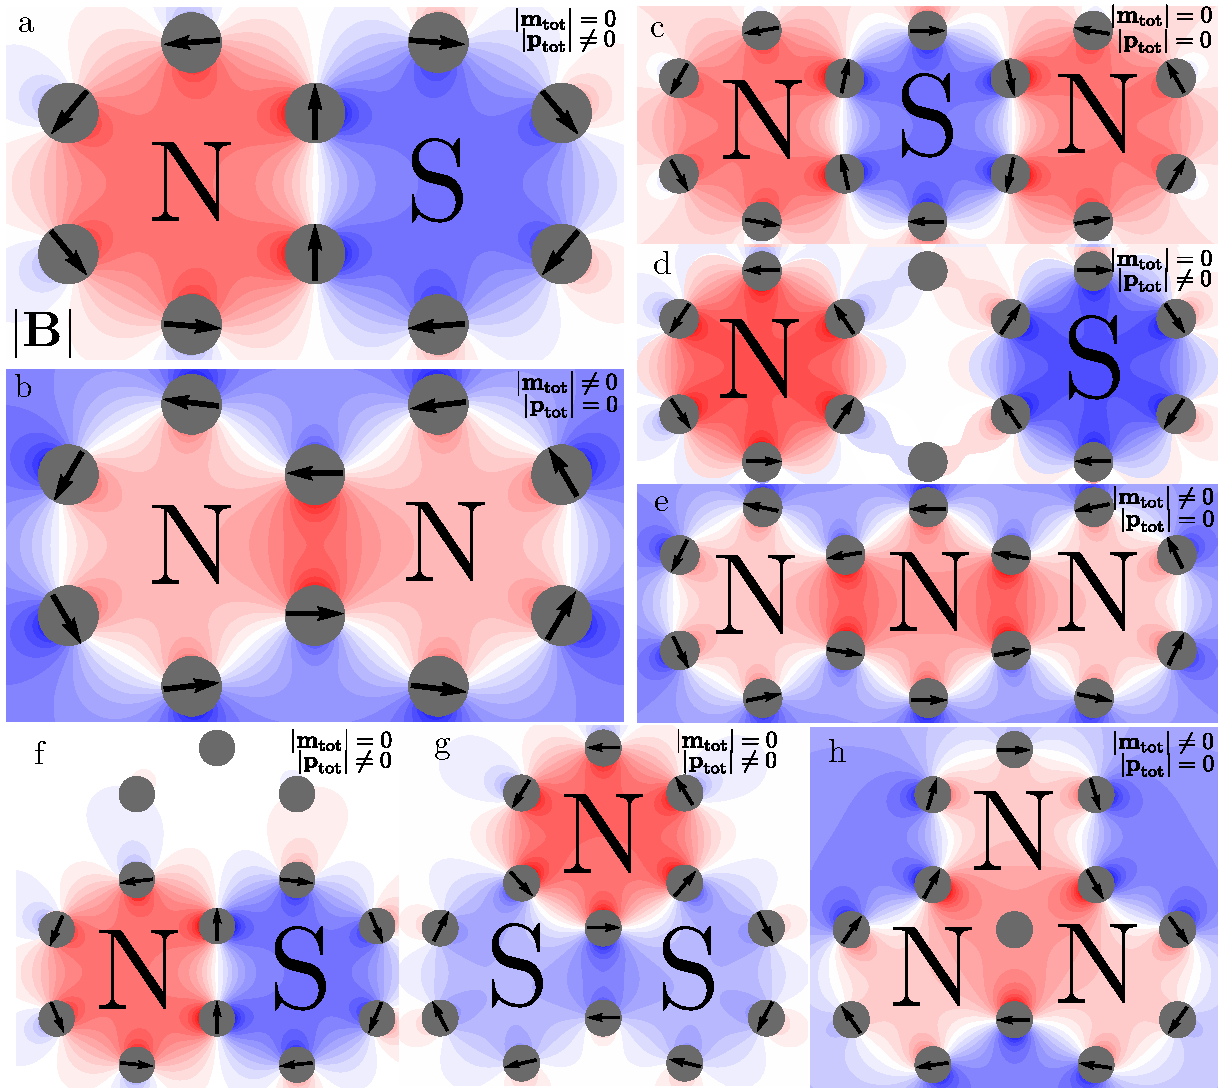
\includegraphics[width=6in]{fields_new_arrows.pdf}
\caption{Magnetic fields produced by each of the magnetic eigenmodes of the twomer (a and b), 1D threemer (c, d, and e), and 2D threemer (f, g, and h). The magnetic field distributions and orientation of electric dipoles can be used to determine whether each magnetic mode is magnetically or electrically bright or dark. Red regions are labeled ``N'' for ``North'' and ``S'' for ``South'' in reference to the north and south poles of a magnet. Interestingly, each oligomer supports exactly one magnetically bright mode (b, e, h) that will couple to the magnetic, rather than the electric, field of light. That this mode's dipole moment is out of the plane of the oligomer allows it to be excited mutually with the electric dipole modes.}
\label{field_plots}
\end{figure}

\section*{Results and Discussion}
Using Equation~\ref{eom} to build and solve a system of equations results in the eigenvalues and eigenvectors for each mode of the oligomers. Figure~\ref{field_plots} shows the oligomers, the dipole moments on each sphere, and the magnetic field distribution of each magnetic mode, computed from\cite{jackson_classical_1999}

\begin{equation}
\textbf{B}_{\textrm{tot}} = \frac{\omega^2}{c^2}\sum_{j}(\hat{\textbf{n}}_{j}\times\textbf{p}_{j})\frac{e^{\textrm{i}\omega r_j/c}}{r_j}\left(1 - \frac{c}{\textrm{i}\omega r_{j}}\right).
\label{magnetic_field}
\end{equation}

\noindent From the magnetic field distributions and the orientation of electric dipoles, some key observations can be made about the magnetic modes. Each magnetic oligomer supports exactly one magnetically bright mode and at least one electrically bright closed-loop mode. Furthermore, the magnetically bright and electrically bright modes are orthogonal to each other, implying that they can be either mutually excited or exclusively excited by the proper polarization of light. Furthermore, this implies that the magnetically bright mode will radiate a different pattern than the in-plane electric modes of the oligomers. These details will be significant in the discussion of observables and applications, as they lead to stark differences in the radaition pattern of light scattered by the oligomer.

The model can now be used to show how properties such as scale of the oligomer and separation distance between MNPs impact the eigenvalues. To do this, a nearest neighbor distance is defined as $r_{\textrm{nn}} = (s+2)r_0$ where $r_0$ is the particle radius and $s$ is the face-to-face distance in units of $r_0$. Figure~\ref{scaling}a shows the magnetic eigenmode frequencies as a function of oligomer scale. This is calculated by fixing the parameter $s=1$ and varying $r_0$ from 1 nm to 30 nm. It can be seen that the eigenmodes of each oligomer change order mutliple times as a function of size. Interestingly, when the oligomers are small they preserve the quasistatic ordering predicted by previous work\cite{Cherqui2014}. As the oligomers grow larger, the spectral ordering changes, a prediction not made by the quasistatic model. This is the result of incorporation of retardation effects, which will be made clearer in Figure~\ref{scaling}b.

\begin{figure}
\centering
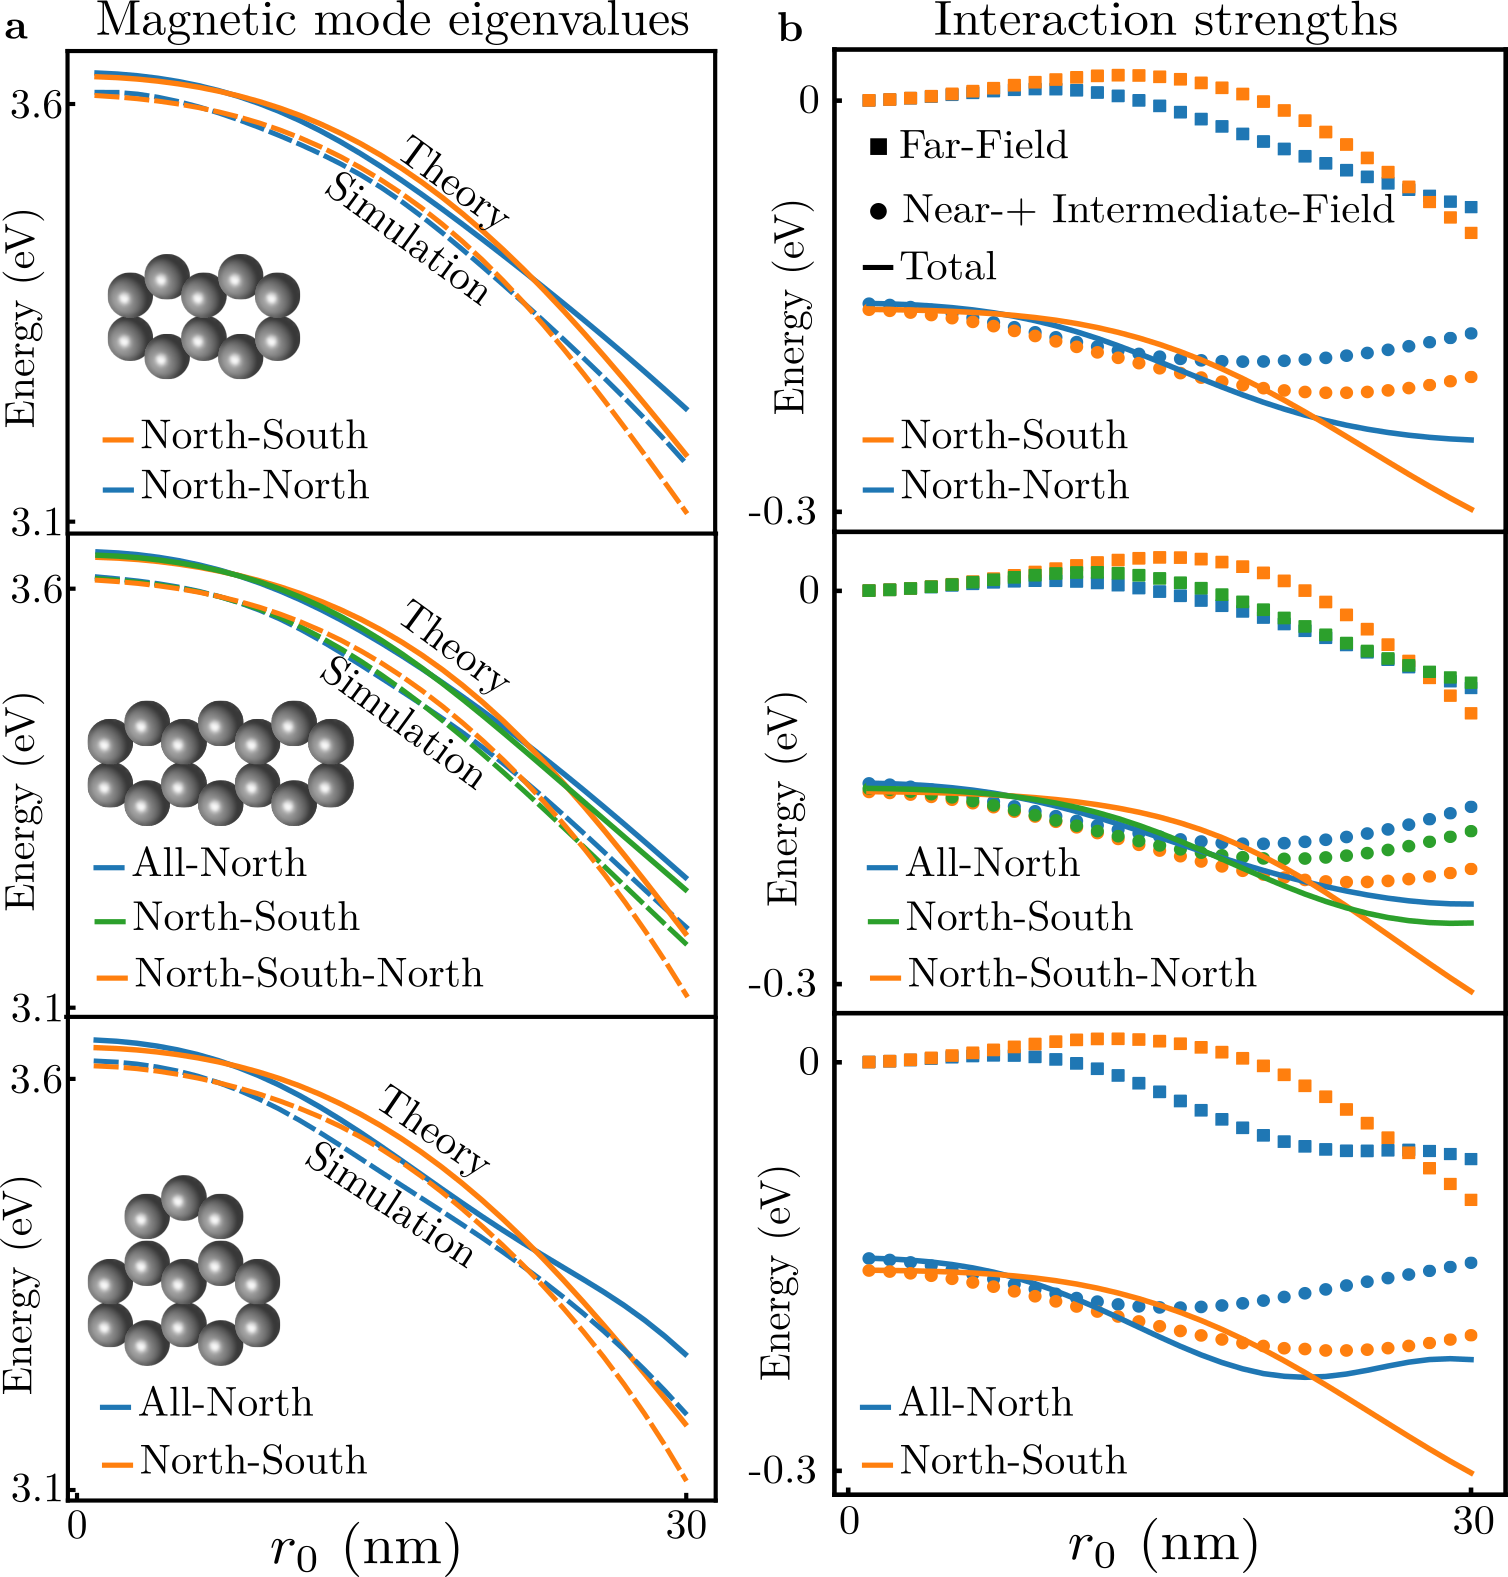
\includegraphics[width=6in]{scale_eigs.png}
\caption{Theoretical and simulated magnetic mode eigenvalues (a) and total, near plus intermediate, and far interaction strengths (b) plotted as a function of $r_0$, with interparticle distances scaling up. Each row corresponds to one of the oligomer systems studied in this work as pictured on the left. In column (a), note that the eigenvalues all decrease with increasing $r_0$, but the eigenvalues cross at 5 nm and 21 nm. This is corroborated by full-wave simulation (dashed lines). Interestingly, these crossings are mirrored in (b) by the fluctuations in the far-field (squares) interaction. By themselves, the near- and intermediate-fields (circles) would never contribute any mode crossings to the total interaction (solid). Due to the opposite inflection of the far-field interaction, however, the crossings become possible.}
\label{scaling}
\end{figure}

In order to more fully explain the effects of incorporating retardation, Figure~\ref{scaling}b shows the total interaction strength, the sum of the near- and intermediate-field interaction strengths, and the far-field interaction strength for each of the closed-loop magnetic modes of the oligomers. In other words, this is the computation of $U_{\textrm{int}} = \sum_{i}\textbf{p}_i \cdot \textbf{E}_{\textrm{tot}}$ for a set of eigenvectors corresponding to each of the closed-loop magnetic modes, where $\textbf{E}_{\textrm{tot}}$ is the electric field of all of the dipoles except the $i^{\textrm{th}}$. Because there are no crossings exhibited in the near- and intermediate-field terms, and because the far-field term exhibits the opposite behavior of the other terms, it can be seen that inclusion of the far-field term results in spectral switching of the eigenmodes. This is because, as can be seen in Equation~\ref{dipoledipole}, the far-field term contributes the opposite ordering to the dyadic structure of the tensor. In other words, the far-field term is 180 degrees out of phase with the near- and intermediate-field terms, and therefore accounts for the ability of the modes to switch order.

Aggregate scale is not something that can be easily manipulated in real time in a laboratory, as it would require the refrabrication of a different aggregate for each experiment. However, recent research has focused on the ability of DNA and polymers to change shape and size in response to stimuli such as heat and pH\cite{DanLuo2009,NaLiu2017,Ginger2017,odom_lasing,Yang2016}. Specifically, these techniques have been used to continuously and reversibly tune the aggregation scheme or environment of a MNP array. Applying these concepts to small magnetic oligomers reveals a high degree of tunability in not only the eigenvalues but their ordering.

\begin{figure}
\centering
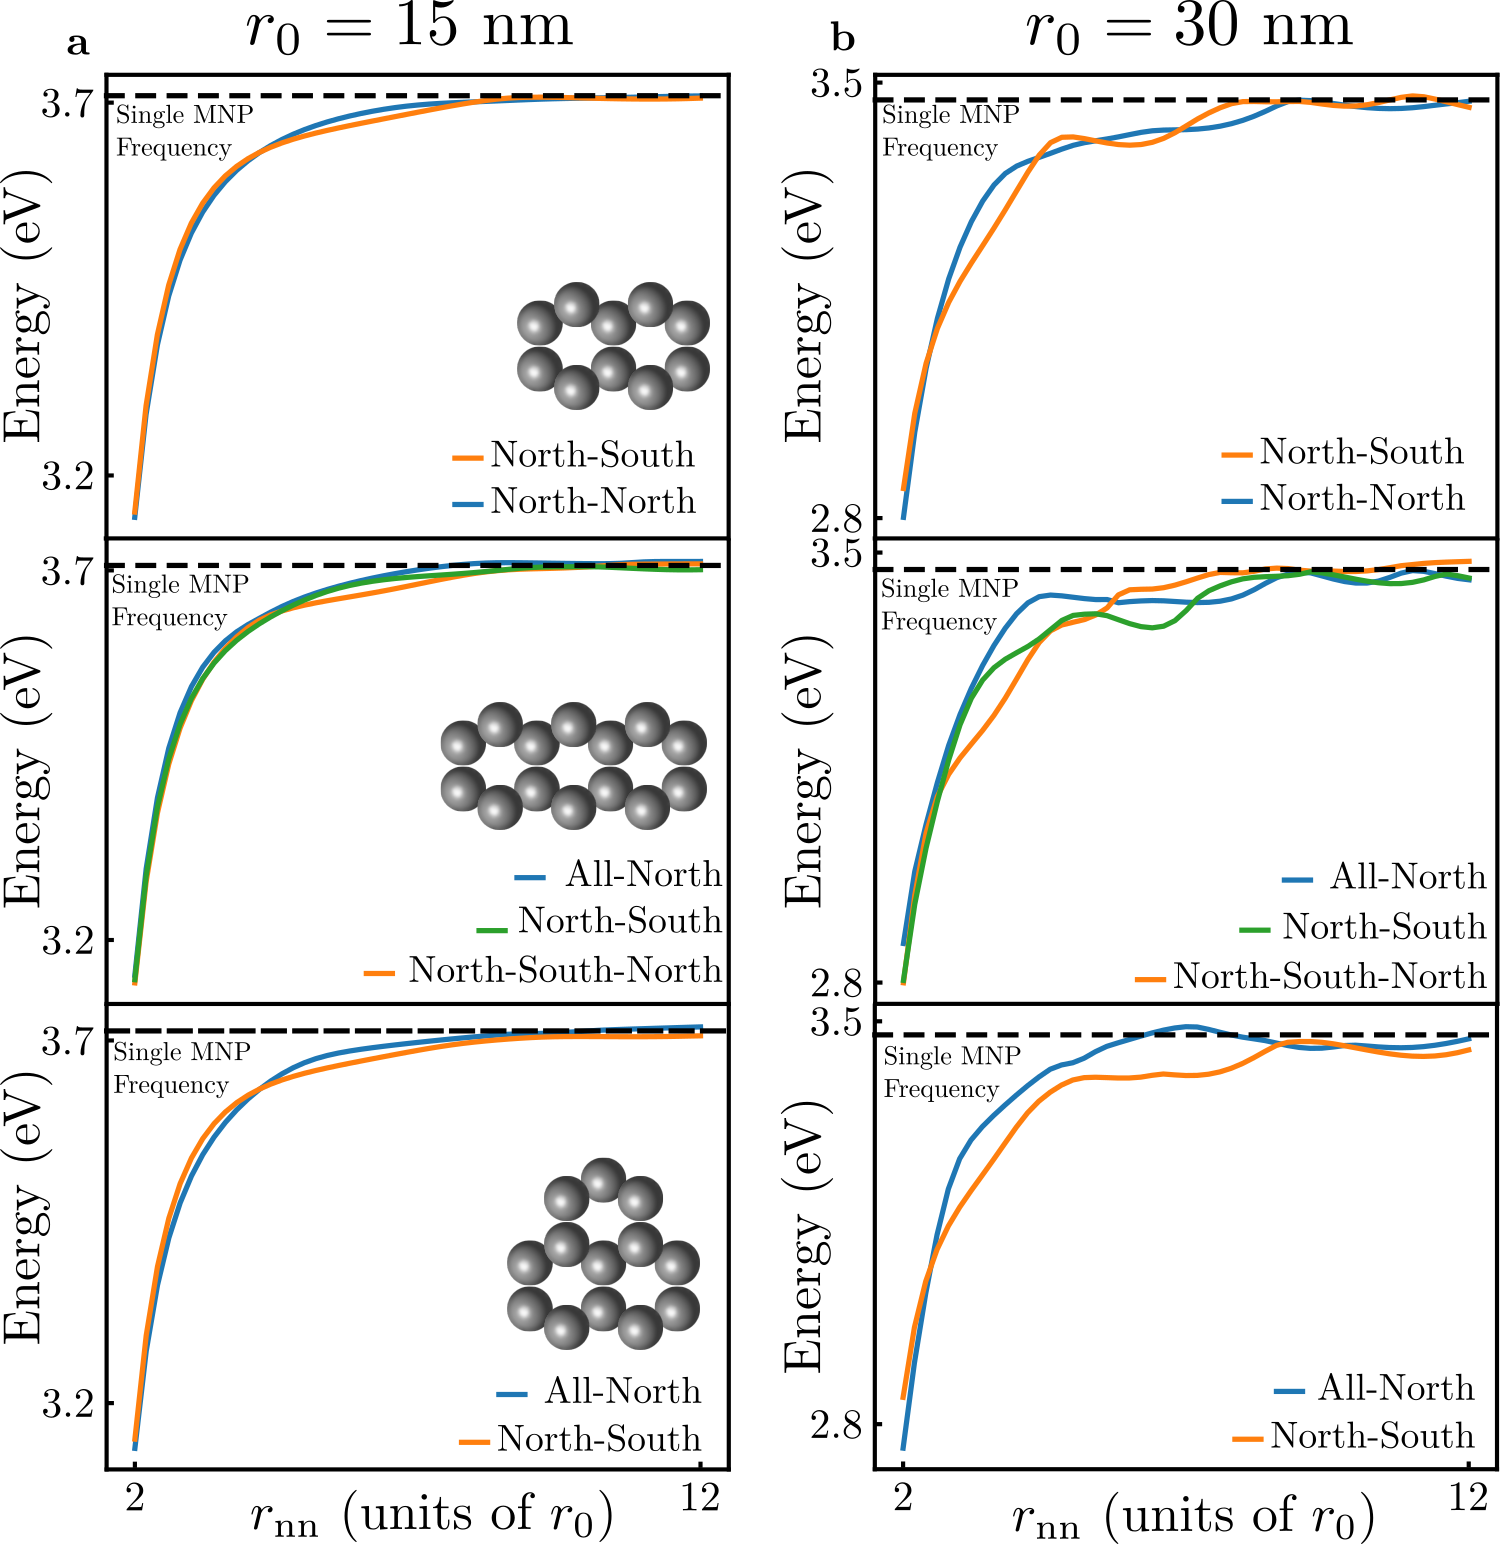
\includegraphics[width=6in]{spacing_study.png}
\caption{Magnetic mode eigenvalues as a function of increasing nearest-neighbor distance for the twomer (first row), 1D threemer (second row), and 2D threemer (third row). For all of the oligomers, the eigenvalues approach the single MNP frequency (black dashed lines) at large separation distances. When the constituent MNPs are 15 nm in radius (column a), the eigenvalues cross minimally and level off to the single MNP frequency rapidly. However, for MNPs of 30 nm in radius (column b) the eigenvalues exhibit larger splittings, more crossings, and larger amplitude oscillations as a function of increasing distance. This is evidence of the increased importance of retardation effects for larger-sized particles at larger distances from each other.}
\label{spacing}
\end{figure}

Figure~\ref{spacing} shows the eigenvalues of each closed-loop mode of the oligomesrs as a function of face-to-face distances for particles of 15 (a) and 30 (b) nm. As the space between particles increases, the magnetic modes collectively increase in energy, tending towards the single plasmon resonant frequency. This is expected, as in the limit that the particles are infinitely far apart they should not interact (see Equation~\ref{dipoledipole}). The eigenvalues appear to cross and exhibit low-amplitude oscillations for both particle sizes, but the crossings and oscillations are much more pronounced for the 30 nm particles. This is evidence of real time tunability and versatility and, more importantly, it implies an overall size dependence to the impact of retardation effects. Comparing the behavior of the smaller particles and the larger particles shows that retardation effects, as expected, play a more important role in aggregates that are both composed of larger particles and span larger distances. As a result, it can be seen that utilizing and understanding the role of retardation effects can lead to increased versatility of magnetic plasmon oligomers.

There is a drawback in this line of reasoning, however. The splitting between the magnetic modes is very small, on the order of hundredths of electron volts, tenths at the most. Due to natural broadening of the plasmonic modes with increasing particle size, it can be difficult to pick apart these modes in optical spectra. In order to fully utilize magnetic oligomers, a technique is required to unravel these overlapping modes. As previously mentioned, the all in-phase magnetic modes scatter light in different directions than the in-plane electric modes (see Figure~\ref{field_plots}). This distinctive radiation pattern can be detected\cite{Polman2014,Smith2014}, and it will be shown that it can be used as a measure of the importance of retardation effects. Furthermore, because the magnetic and electric dipole moments have orthogonal orientations, they are mutually excitable and interfere with each other to produce directional radiation\cite{Kivshar2012,Tsutomu2017}.

The following discussion stems from calculations performed using a full-wave Maxwell's equations solver\cite{Hohenester2012}. The results of those calculations are shown in Figures~\ref{polar_plots_yz} and~\ref{beaming}. As in the figures, polarizing an incident light wave such that its magnetic field threads the rings of a magnetic oligomer and its electric field is in the plane of the oligomer along its y-axis allows both the excitation of the closed-loop, in-phase magnetic mode and all of the in-plane electric modes oriented along the electric field.

\begin{figure}
\centering
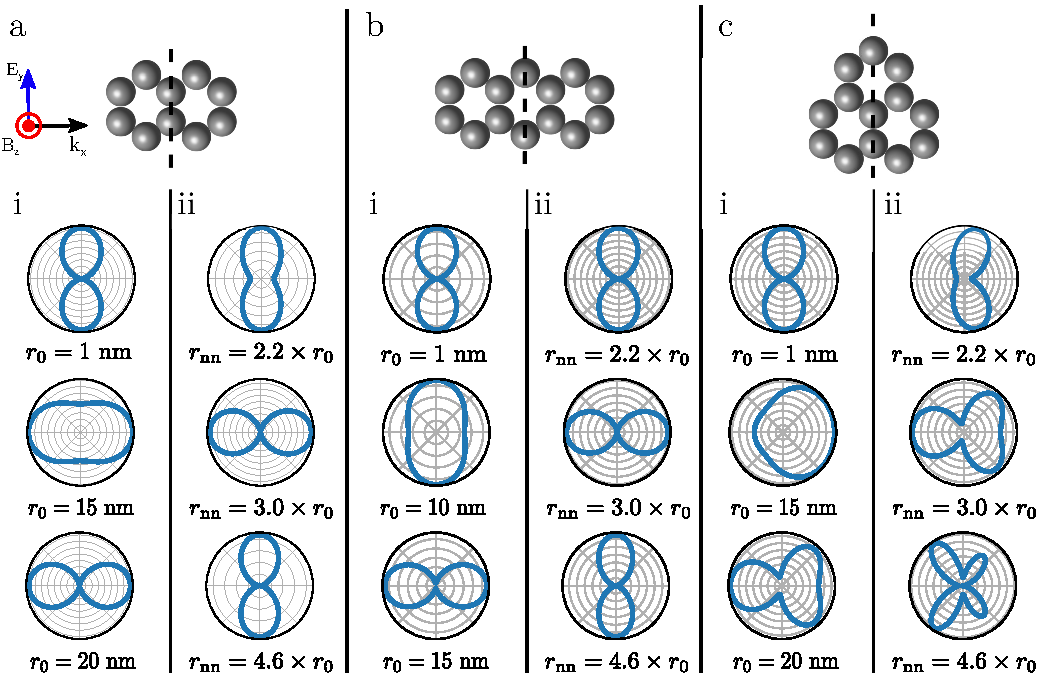
\includegraphics[width=6in]{polar_plots_yz.pdf}
\caption{Differential scattering plots for the twomer (a), 1D threemer (b), and 2D threemer (c) computed in the plane along the dotted lines in each diagram (the E,B or y,z plane). In the columns marked i the differential scattering is computed at the magnetic plasmon frequency with changing scale, and in the columns marked ii the differential scattering is computed at a fixed frequency with fixed particle radius as a function of increasing spacing. The scale calculations show that at small sizes, the radiation pattern is dominated by the electric dipole, which scatters heavily in the z-direction and not at all in the y-direction. At large sizes, the magnetic dipole dominates, as the scattering pattern changes to show heavy radiation in the y-direction and very little in the z-direction. The spacing calculations show that when looking at a fixed frequency, the magnetic oligomers can be brought into and out of their magnetic dipole resonance, seen for all three systems at $r_{\textrm{nn}}=3.0\times r_0$. Interestingly the scattering patterns of the 2D threemer are biased towards the y-direction. Due to the degeneracy in its electric dipole moments, the x-directed dipoles can be weakly excited with this polarization of light and, at larger sizes, can influence the radiation pattern.}
\label{polar_plots_yz}
\end{figure}

Figure~\ref{polar_plots_yz} displays the scattered power of the oligomers in the plane containing the electric field vector and the magnetic field vector, the yz-plane. It can be seen that at small sizes (columns marked i) the electric dipole radiation dominates the differential power, but with increasing size the magnetic dipole wins. This is evidence that the magnetic dipole moments of the oligomers only impact the oligomer's optical properties when the system is too large to be described by the quasistatic limit. In other words, when retaradtion effects are important, so too are the magnetic plasmons. Furthermore, computing the differential scattering at a fixed frequency with fixed MNP radius and changing the spacing of the oligomer (columns marked ii) results in a scattering pattern that detects when the magnetic mode is in resonance. This is direct evidence of the utility of magnetic plasmon oligomers as switches because the radiation pattern can be directly tuned and detected.

\begin{figure}
\centering
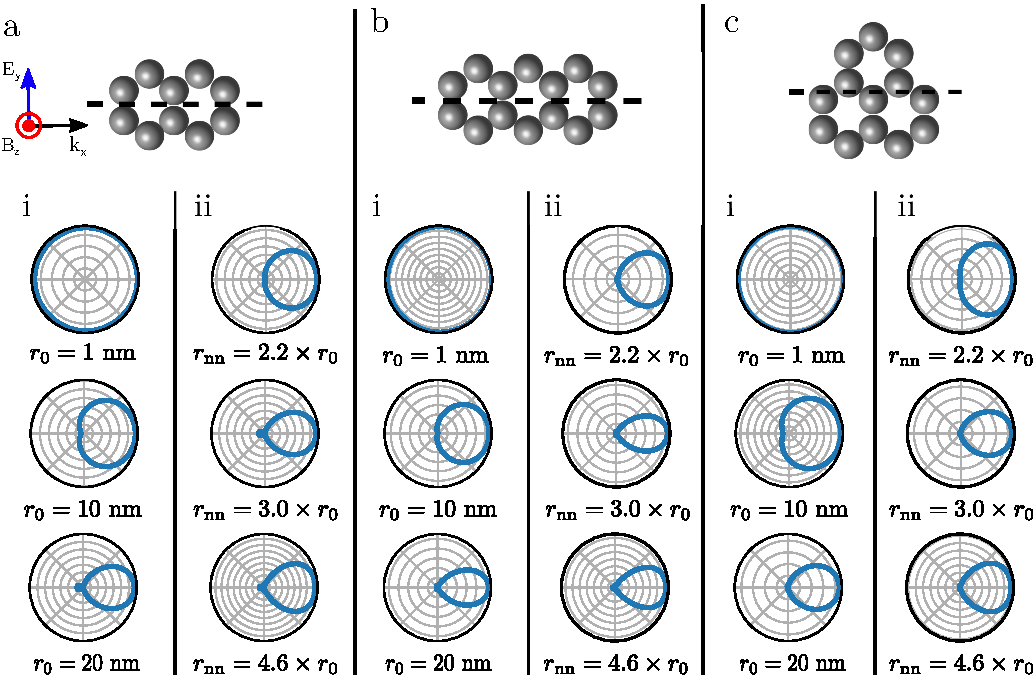
\includegraphics[width=6in]{beaming.pdf}
\caption{Differential scattering plots for the twomer (a), 1D threemer (b), and 2D threemer (c) computed in the plane along the dotted lines in each diagram (the k,B or x,z plane). In the columns marked i the differential scattering is computed at the magnetic plasmon frequency with changing scale, and in the columns marked ii the differential scattering is computed at a fixed frequency with fixed particle radius as a function of increasing spacing. The scale calculations show that at small sizes, the radiation pattern is dominated by the electric dipole, which scatters nearly isotropically in the x- and z-directions. At large sizes, the magnetic dipole begins to influence the radiation pattern, evidenced by the biasing of the radiation pattern to the x-direction. This is an indication of unidirectional scattering, very likely brought about by the interference of the magnetic and electric dipoles. The spacing calculations show that once the oligomers are large enough to exhibit magnetic-electric interference, it is difficult to turn the interference off. This can be seen in the differential scattering patterns as they remain unidirectional or somewhat biased to one direction at all spacings. However, there is a spacing at which the radiation unidirectionality is optimized.}
\label{beaming}
\end{figure}

Upon switching the plane of detection in these radiation pattern calculations, another interesting property of magnetic oligomers comes to light: their ability to emit directional radiation. Figure~\ref{beaming} displays the radiation patterns collected in the plane defined by the light propagation direction and the impinging magnetic field (the xz-plane, see dotted lines). At small sizes (columns marked i) each magnetic oligomer exhibits nearly isotropic radiation due to the scattering of the electric dipole. However, as the oligomers grow, the radiation begins to bias towards the propagation direction. Interestingly, changing the spacing at constant size and frequency doesn't greatly impact the radiation patterns (columns marked ii). These pieces of information taken together point to the interference of the magnetic dipole modes and the electric dipole modes. This is predicted for metal-semiconductor core-shell nanoparticles, but not for magnetic oligomers\cite{Kivshar2012}, creating an impetus for a simple model to explain these phenomena.

These scattering properties of magnetic plasmon oligomers are interesting in that they are observable and applicable. However, what is missing is an intuitive understanding of why these systems should produce directional radiation. A few hypothetical models are proposed in the Future Work section. Barring that, this work has shown that magnetic plasmon oligomers exhibit tunable spectral ordering of their closed-loop magnetic modes. Additionally, it has been shown computationally that magnetic plasmon oligomers scatter light in different directions depending on morphological parameters. This directionality can be turned on and off both by moving the MNPs and by rotating the laser polarization, a result which implies switching and sensing applications for magnetic plasmon oligomers.

\section*{Future Work}
Presented here are two hypothetical models of the differential power of the magnetic plasmon oligomers. The first comes from computing the electric and magnetic fields scattered by each dipole in the aggregate. The second comes from approximating each ring as a unit cell with a distinct magnetic and electric dipole moment\cite{Kivshar2012}.

Computing the differential power of the full aggregate requires\cite{jackson_classical_1999}

\begin{multline}
\frac{dP}{d\Omega} = \frac{c}{8\pi}\textrm{Re}\left[r^2 \hat{\textbf{n}}\cdot \sum_i \textbf{E}_i \times \sum_j \textbf{B}_j\right]\\
= \frac{\omega^4}{8\pi c^3}\textrm{Re}\left[\hat{\textbf{n}}\cdot \left(\sum_i \left(\frac{\textbf{r}-\textbf{r}_i}{r}\times\textbf{p}_i\right)\times\frac{\textbf{r}-\textbf{r}_i}{r}\right)e^{\textrm{i}\omega|\textbf{r}-\textbf{r}_i|/c} \times \sum_j\left(\frac{\textbf{r}-\textbf{r}_j}{r}\times\textbf{p}_j\right)e^{\textrm{i}\omega|\textbf{r}-\textbf{r}_j|/c}\right]
\label{diff_power_full}
\end{multline}

\noindent where at every point $\textbf{r}$ on the flux screen the fields scattered by each dipole located at positions $\textbf{r}_i$ are added together before the cross product is taken. There are two relevant limits to take: one in which the loop of dipoles is very small compared to the distance to the detector ($|\textbf{r}-\textbf{r}_i| \approx r$) and one in which the loop is finite in size ($|\textbf{r}-\textbf{r}_i| \approx r-\hat{\textbf{n}}\cdot\textbf{r}_i$). Taking the first limit results in

\begin{equation}
\frac{dP}{d\Omega} = \frac{\omega}{2\pi c r^2}|\textbf{m}|^2\textrm{sin}^2\theta
\label{mag_dp}
\end{equation}

\noindent a term which decays to zero for a flux screen at infinity. Here, $\textbf{m} = (N\omega Rp/2c)\hat{\textbf{z}}$ with $R$ the radius of one ring of nanoarticles.\cite{Cherqui2014,jackson_classical_1999}. Allowing the loop to have finite size, however, introduces phase effects. It is these that contribute to the overall radiation of the loops of dipoles. Keeping the exponential terms and again letting the magnetic dipole terms decay to zero gives

\begin{equation}
\frac{dP}{d\Omega} = \frac{\omega^4}{8\pi c^3}\sum_{ij}\left[\textbf{p}_i\textbf{p}_j - (\textbf{p}_i\cdot\hat{\textbf{n}})(\textbf{p}_j\cdot\hat{\textbf{n}})\right]\textrm{e}^{\textrm{i}\omega\hat{\textbf{n}}\cdot(\textbf{r}_j-\textbf{r}_i)/c}.
\label{dipoles_only_dp}
\end{equation}

\noindent From this, it can be seen that the radiation pattern of a collection of dipoles, regardless of arrangement, is dependent only on the orientations and locations of the dipoles in relation to one another. This equation is not immediately intuitive, however, and does not paint a physical picture of how the magnetic modes interfere with one another.

The second approach stems from the demonstrated ability of a magnetic dipole moment and an electric dipole moment to interfere and produce directional radiation\cite{Kivshar2012}. Applying this concept to magnetic oligomers results begins with\cite{schwinger1998classical}

\begin{multline}
\frac{dP}{d\Omega} = \frac{\omega^4}{4\pi c^3}\left[\hat{\textbf{n}}\times(\textbf{p} - \hat{\textbf{n}}\times\textbf{m})\right]^2= \frac{\omega^4}{4\pi c^3}\left[(\hat{\textbf{n}}\times\textbf{p})^2 + (\hat{\textbf{n}}\times\textbf{m})^2 + 2\hat{\textbf{n}}\cdot(\textbf{p}\times\textbf{m})\right].
\label{schwing_dP_1}
\end{multline}

\noindent Using the same light polarization in Figures~\ref{polar_plots_yz} and ~\ref{beaming} generates an electric dipole in the y-direction and a magnetic dipole in the z-direction associated with each ring of nanoparticles in the oligomer. Enforcing these conditions, Equation~\ref{schwing_dP_1} becomes

\begin{equation}
\frac{dP}{d\Omega}=\frac{\omega^4}{4\pi c^3}\sum_{i}\left[p_i^2(1 - (\hat{\textbf{n}}\cdot\hat{\textbf{y}})^2) + m_i^2(1 - (\hat{\textbf{n}}\cdot\hat{\textbf{z}})^2) + 2d_im_i(\hat{\textbf{n}}\cdot\hat{\textbf{x}})\right],
\label{schwing_dP_2}
\end{equation}

\noindent showing that an asymmetric interference term arises from the cross product of the magnetic and electric dipole.Equation~\ref{schwing_dP_2} shows that if either of the dipole moments is far greater than the other, that one will dominate the scattered power, but if they are nearly commensurate in strength, the unidirectionality will be optimized. This expression intuitively and qualitatively agrees with the data presented in Figures~\ref{polar_plots_yz} and~\ref{beaming}, but whether or not this is a good approximation has not been verified.

Beyond computing radiation patterns, the model of magnetic plasmon oligomers will be useful for other future projects. Incorporating a time component and initial conditions into the model will result in the ability to prepare a magnetic or electric plasmon and study its propagation through some oligomeric aggregate. This is especially interesting in light of Figures~\ref{scaling} and ~\ref{spacing}. One question that can be asked is whether the initial frequency of a magnetic plasmon impacts its phase as it propagates through an aggregate. Another question is how the propagation times and lengths of electric and magnetic plasmons on the same oligomer compare to each other.

Another application of the model proposed in this work is investigation of arrays of semiconductor nanocrystals (SNCs). SNCs are of interest to the plasmonics community because they offer yet another knob to turn, specifically offering direct control over the electron density in the nanocrystals\cite{Gamelin2014}. SNCs have been shown to produce narrow plasmon resonances in the infrared. It has been previously proposed that magnetic plasmon oligomers composed of SNCs are the perfect medium to couple to the magnetic dipole transition in Yb,Er nanocrystals. It is thought that a metamaterial of this composition, when combined in a photovoltaic device, can be a route to surpassing the Shockley-Quiesser limit through upconversion of infrared photons into blue or violet light.

With a versatile, accurate, and fast model that contains many knobs to turn, these explorations should be both possible and fruitful. They are the next steps in turning magnetic plasmon oligomers into useful and functional nanoscale technologies.

%%%%%%%%%%%%%%%%%%%%%%%%%%%%%%%%%%%%%%%%%%%%%%%%%%%%%%%%%%%%%%%%%%%%%
%% The appropriate \bibliography command should be placed here.
%% Notice that the class file automatically sets \bibliographystyle
%% and also names the section correctly.
%%%%%%%%%%%%%%%%%%%%%%%%%%%%%%%%%%%%%%%%%%%%%%%%%%%%%%%%%%%%%%%%%%%%%
\bibliography{references}
\end{document}
